%%%%%%%%%%%%%%%%%%%%%%%%%%%%%%%%%%%%%%%%%
% Beamer Presentation
% LaTeX Template
% Version 1.0 (10/11/12) 
%
% This template has been downloaded from:
% http://www.LaTeXTemplates.com
%
% License:
% CC BY-NC-SA 3.0 (http://creativecommons.org/licenses/by-nc-sa/3.0/)
%
%%%%%%%%%%%%%%%%%%%%%%%%%%%%%%%%%%%%%%%%%

%----------------------------------------------------------------------------------------
%	PACKAGES AND THEMES
%----------------------------------------------------------------------------------------

\documentclass{beamer}

\mode<presentation> {
%\mode<handouts> {
%\mode<article> {


% The Beamer class comes with a number of default slide themes
% which change the colors and layouts of slides. Below this is a list
% of all the themes, uncomment each in turn to see what they look like.


%\usetheme{default}
%\usetheme{AnnArbor}
%\usetheme{Antibes}
%\usetheme{Bergen}
%\usetheme{Berkeley}
%\usetheme{Berlin}
%\usetheme{Boadilla}
\usetheme{CambridgeUS}
%\usetheme{Copenhagen}
%\usetheme{Darmstadt}
%\usetheme{Dresden}
%\usetheme{Frankfurt}
%\usetheme{Goettingen}
%\usetheme{Hannover}
%\usetheme{Ilmenau}
%\usetheme{JuanLesPins}
%\usetheme{Luebeck}
%\usetheme{Madrid}
%\usetheme{Malmoe}
%\usetheme{Marburg}
%\usetheme{Montpellier}
%\usetheme{PaloAlto}
%\usetheme{Pittsburgh}
%\usetheme{Rochester}
%\usetheme{Singapore}
%\usetheme{Szeged}
%\usetheme{Warsaw}

% As well as themes, the Beamer class has a number of color themes
% for any slide theme. Uncomment each of these in turn to see how it
% changes the colors of your current slide theme.

%\usecolortheme{albatross}
\usecolortheme{beaver}
%\usecolortheme{beetle}
%\usecolortheme{crane}
%\usecolortheme{dolphin}
%\usecolortheme{dove}
%\usecolortheme{fly}
%\usecolortheme{lily}
%\usecolortheme{orchid}
%\usecolortheme{rose}
%\usecolortheme{seagull}
%\usecolortheme{seahorse}
%\usecolortheme{whale}
%\usecolortheme{wolverine}

%\setbeamertemplate{footline} % To remove the footer line in all slides uncomment this line
%\setbeamertemplate{footline}[page number] % To replace the footer line in all slides with a simple slide count uncomment this line

%\setbeamertemplate{navigation symbols}{} % To remove the navigation symbols from the bottom of all slides uncomment this line
}

\usepackage{graphicx} % Allows including images
\graphicspath{{../figures}}
\usepackage{booktabs} % Allows the use of \toprule, \midrule and \bottomrule in tables
\usepackage{amsmath, amssymb, amsthm, gensymb,mathrsfs}%,eufrak}
\usepackage{hyperref}
\usepackage{tabularx}
\usepackage{longtable}
\usepackage{makecell}
\usepackage{multicol}
\usepackage{physics}

\newcommand{\uvec}[1]{\textbf{#1}}

\newcounter{excounter}
%\renewcommand{\thefpcounter}{\thechapter.\arabic{fpcounter}}
%\renewcommand{\thefpcounter}{\thesection.\arabic{fpcounter}}
\renewcommand{\theexcounter}{\arabic{excounter}}

\newtheorem{teorema}{Teorema}[section]
\newtheorem{definicio}{Definició}[section]

\usepackage[lastexercise]{exercise}

\graphicspath{{../figures}}

%----------------------------------------------------------------------------------------
%	 TITLE PAGE
%----------------------------------------------------------------------------------------

\title[Introduction]{Brief introduction to Python\\\small (with a Structural Bioinformatcs bias)} % The short title appears at the bottom of every slide, the full title is only on the title page

\author{Jordi Villà i Freixa} % Your name
\institute[FCTE] % Your institution as it will appear on the bottom of every slide, may be shorthand to save space
{
Universitat de Vic - Universitat Central de Catalunya \\
Study Abroad\\ % Your institution for the title page
\medskip
\textit{jordi.villa@uvic.cat}\\ % Your email address
\copyright Michael A. Johnston 2007; JVF 2007-2023 
}
%\date{\today} % Date, can be changed to a custom date
\date{course 2023-2024}
\logo{
\includegraphics[width=.1\textwidth]{FCTE}}
\begin{document}


\begin{frame}
  \titlepage % Print the title page as the first slide
\end{frame}

\begin{frame}
  \frametitle{Disclaimer}
  This material was originally created by Michael A. Johnston and myself as the course material for a general introduction to Python at the MSc on Bioinformatics for Health Sciences at the Universitat Pompeu Fabra. The material has not been updated much since then, although the original syntax on Python 2.x has been ported to Python 3.x. However, it is likely that some deprecated material is still present here. I would appreciate if you let me know in case you detect some. 
\end{frame}


%%%%%%%%%%%%%%%%%%%%%%%%%%%%%%%%%%
\part{Framework}
%%%%%%%%%%%%%%%%%%%%%%%%%%%%%%%%%%
% To define a frame containing the layout of the presentation
\begin{frame}
\tableofcontents
\end{frame}

\section{Intro}
\section{Functional programming}

\begin{frame}[containsverbatim]
\frametitle{Programming}
\begin{itemize}
\item Programs operate on various "data types": integers, strings, doubles
\item Concept of variable and assignment: 
\begin{lstlisting}
Age = 3
\end{lstlisting}
\item Expresions create and process data:
\begin{lstlisting}
x>3
y=x*2
\end{lstlisting}
\item Control of flow: conditioning testing (if, else) and iterations (for, while loops)
\item Procedural programming: using functions to divide your program into logical chunks
\end{itemize}
Basic programming concepts! Only syntax change.
\end{frame}

\begin{frame}
\frametitle{Python}
\begin{itemize}
\item Dynamical, interpreted, object oriented programming language
\item Software quality: designed to be readable, coherent and maintainable
\item Developer productivity: very compact code (20-33\% of the size of the corresponding java/C code): less code $\rightarrow$ less to debug $\rightarrow$ less to maintain $\rightarrow$ less to learn
\end{itemize}
Some help: \url{http://greenteapress.com/thinkpython/thinkpython.html}
\end{frame}

\begin{frame}
\frametitle{The subject}
About making it quicker for you and others to write, maintain and extend programs. To do so:
\begin{itemize}
\item Reduce the time spent in programming \& debugging: OOP, testing
\item Make it easy to extend your program: code reuse (OOP)
\item Reduce the time for others to understand your program: documentation, program readability
\end{itemize}
\end{frame}

\begin{frame}[containsverbatim]
\frametitle{The Python interpreter}
\begin{Verbatim}
  Python 3.11.4 (main, Jul  5 2023, 13:45:01) [GCC 11.2.0] on linux
  Type "help", "copyright", "credits" or "license" for more information.
  >>> print(2+3)
  5
\end{Verbatim}
Alternatively, you can store code in a file and use the interpreter to execute the contents of the file. Such a file is called a script. For example, you could use a text editor to create a fle named \texttt{dinsdale.py} with the following contents: 
\begin{lstlisting}
print(2+3) 
\end{lstlisting}
By convention, Python scripts have names that end with .py. 
\end{frame}

\begin{frame}
\frametitle{IDLE or other IDEs}
\begin{itemize}
\item IDLE is the Python Integrated Development Environment: \url{http://docs.python.org/library/idle.html}
\begin{itemize}
\item First step in making it easier to write Python code
\item Syntax highlighting
\item Code completion
\item Inline documentation
\item Many other useful features
\end{itemize}
\item Eclipse is... "an open extensible IDE for anything and nothing in particular". Extension to Python through PyDEV
\item Visual code as the tool of choice, but also PyCharm, Spyder and Jupyter and other
\item but check also other possibilities: \url{http://wiki.python.org/moin/PythonEditors}
\end{itemize}
\end{frame}

\begin{frame}[containsverbatim]
\frametitle{Structure of a program}
\begin{itemize}
\item Programs are composed of {\em modules}
\item Modules contain statements:
\begin{itemize}
\item Function definitions
\item Control statements (if, while, etc)
\item Variable assignments
\end{itemize}
\item Statements contain expressions:
\begin{lstlisting}
x<3
a=x*x+2
\end{lstlisting}
\item Expressions {\em create and process objects}
\end{itemize}
\end{frame}

\begin{frame}[containsverbatim]
\frametitle{Python keywords}
\label{ref:reserved}
\begin{lstlisting}
and       del     from    not    while 
as        elif    global  or     with 
assert    else    if      pass   yield 
break     except  import  print 
class     exec    in      raise 
continue  finally is      return 
def       for     lambda  try 
\end{lstlisting}
\end{frame}

\begin{frame}[containsverbatim]
\frametitle{Numbers}
\begin{itemize}
\item Types: integer, floating point, long integers, bool (True, False)
\item Basic expression operators \& precedence
\url{http://www.ibiblio.org/g2swap/byteofpython/read/operator-precedence.html}  
\item Conversion: mixed types are converted up, e.g., Integers $\rightarrow$ floating point
\begin{lstlisting}
40+3.14
\end{lstlisting}
\end{itemize}
\end{frame}

\begin{frame}[containsverbatim]
\frametitle{Dynamic typing}
Variable types are decided at runtime
\begin{itemize}
\item Variables are created when you assign values to them
\item Variables {\em refer} to an object, e.g., a number
\item The object has a type; the variable does not
\item When a variable appears in an expression, it is immediately replaced by the object it refers to
\end{itemize}
\begin{example}
\begin{lstlisting}
a=3
\end{lstlisting}
\begin{itemize}
\item Create an object of type integer that represents the number \texttt{3}
\item Create variable \texttt{a} if it does not exist yet
\item link the variable \texttt{a} to the new object \texttt{3}
\end{itemize}
\end{example}
\end{frame}

\begin{frame}
\frametitle{Dynamic typing}
\begin{center}
\only<1>{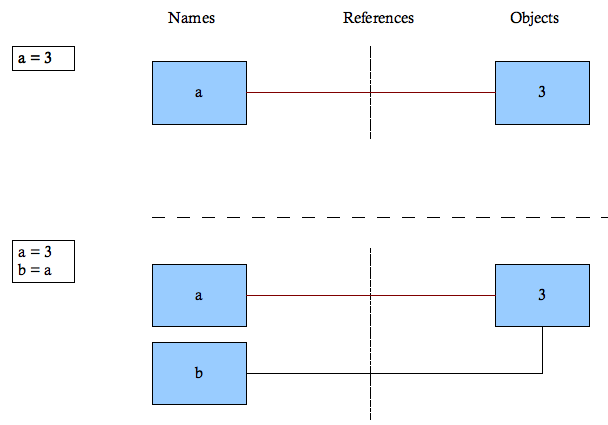
\includegraphics[width=10cm]{dynamic_typing_1}}
\only<2>{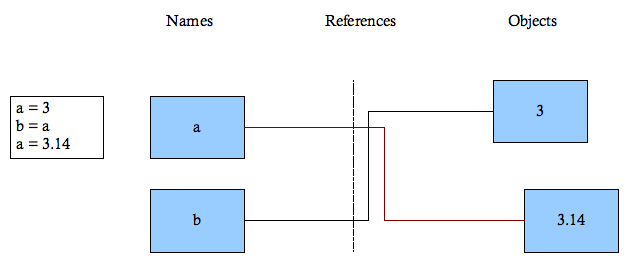
\includegraphics[width=10cm]{dynamic_typing_2}}
\end{center}
\end{frame}

\begin{frame}
\frametitle{Garbage collection}
When no variables are left that reference an object, it is destroyed (automatic memory management)
\begin{center}
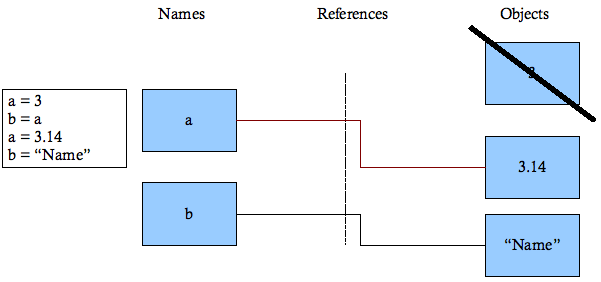
\includegraphics[width=10cm]{dynamic_typing_3}
\end{center}
\end{frame}

\begin{frame}
\frametitle{Modules}
\begin{itemize}
\item Every file containing python code whose name ends in \texttt{.py} is a module
\item A module usually contains a number of items e.g. Variables and functions which you can access. These items are called attributes
\item You load a module using the import statement
\item Just like a number a module is an object
\item You can reload a module after changing it using the \texttt{reload()} function
\item You access modules attributes using the \texttt{.} operator: \texttt{myModule.myAttribute}
\item Modules are the highest level way of organising your program
\item Large programs have multiple module files each of which contains related code
\end{itemize}
\end{frame}

\begin{frame}[containsverbatim]
\frametitle{Documentation}
\begin{itemize}
\item Documentation is one of the core parts of good programming
\item Python contains an inbuilt documentation mechanism using "doc strings"
\item For modules the doc string is the first string in the module file.
\item Doc strings must be enclosed in triple quotes.
\item A modules doc string is accessible through an attribute called \texttt{\_\_doc\_\_}
\end{itemize}
\tiny
\begin{Verbatim}
>>> import os
>>> os.access.__doc__
'access(path, mode) -> 1 if granted, 0 otherwise
Test for access to a file.'
>>>
\end{Verbatim}
\normalsize
\end{frame}

\begin{frame}[containsverbatim]
\frametitle{More docstring examples}
\begin{lstlisting}
def phase_of_the_moon():
  '''
  This function returns a slightly randomized
  integer that shuffles data around in a way
  convenient for the XYZ class.
  '''
  # Working code here.
  return value 
\end{lstlisting}
\end{frame}

\begin{frame}
\frametitle{Module attributes}
\begin{itemize}
\item \texttt{\_\_doc\_\_} is one of four special module attributes
\item The others are:
\begin{itemize}
\item \texttt{\_\_name\_\_} - The module name
\item \texttt{\_\_file\_\_} - The modules file name (complete path)
\item \texttt{\_\_builtin\_\_} - Ignore for now.
\end{itemize}
\item All special names in python begin and end with \texttt{\_\_}
\item You can see all the attributes of a module using the \texttt{dir()} function, which returns a list data type - more on lists later
\end{itemize}
\texttt{dir} returns a list of the attributes and methods of any object: modules, functions, strings, lists, dictionaries... 
\end{frame}

\begin{frame}[containsverbatim]
\frametitle{The import search path}
\begin{lstlisting}
>>> import sys                 
>>> sys.path                   
['', '/usr/local/lib/python2.2', '/usr/local/lib/python2.2/plat-linux2', 
'/usr/local/lib/python2.2/lib-dynload', '/usr/local/lib/python2.2/site-packages', 
'/usr/local/lib/python2.2/site-packages/PIL', 
'/usr/local/lib/python2.2/site-packages/piddle']
>>> sys                        
<module 'sys' (built-in)>
>>> sys.path.append('/my/new/path') 
\end{lstlisting}
\begin{lstlisting}
import sys, os
print ('sys.argv[0] =', sys.argv[0] )            
pathname = os.path.dirname(sys.argv[0])        
print ('path =', pathname)
print ('full path =', os.path.abspath(pathname))
\end{lstlisting}
\end{frame}

\begin{frame}
\frametitle{Function basics}
\url{http://docs.python.org/library/functions.html}
\begin{itemize}
\item We have already seen two functions - \texttt{reload()} \& \texttt{dir()}
\item Functions are defined using the \texttt{def} statement
\item The \texttt{return} statement sends a functions result back to the caller.
\item All code that is in the function must be indented
\item The function ends when the indentation level is the same as the def statement that created it.
\item The functions arguments are given in brackets after the name
\begin{itemize}
\item Note you do not declare types in the argument list!
\item You can use any object as the arguments to a function: e.g. Numbers, modules and even other functions!
\end{itemize}
\end{itemize}
\end{frame}

\begin{frame}
\frametitle{An example function}
\lstinputlisting{../code/function1.py}
\end{frame}

\begin{frame}
\frametitle{Recursivity}
\begin{example}
Write a function for the factorial of a number
\end{example}
\begin{example}
Write a function for counting down from a given integer
\end{example}
\end{frame}

\begin{frame}
\frametitle{Factorial}
\lstinputlisting{../code/factorial.py}
\end{frame}

\begin{frame}
\frametitle{Countdown}
\lstinputlisting{../code/countdown.py}
\end{frame}

\begin{frame}
\frametitle{More on functions}
\begin{itemize}
\item The function is not created until \texttt{def} is executed
\item Like numbers and modules, functions are objects
\item When \texttt{def} executes it creates a function object and associates a name with it.
\end{itemize}
\begin{center}
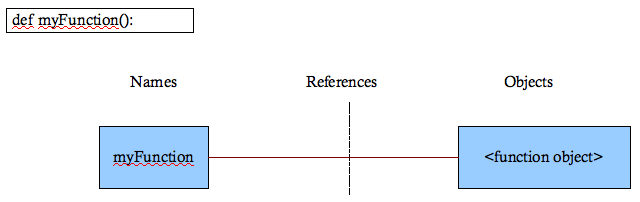
\includegraphics[width=10cm]{functions_1}
\end{center}
\end{frame}

\begin{frame}[containsverbatim]
\frametitle{Argument values}
\begin{lstlisting}
def ask_ok(prompt, retries=4, complaint='Yes or no, please!'):
    while True:
        ok = raw_input(prompt)
        if ok in ('y', 'ye', 'yes'):
            return True
        if ok in ('n', 'no', 'nop', 'nope'):
            return False
        retries = retries - 1
        if retries < 0:
            raise IOError('refusenik user')
        print (complaint)
ask_ok('Do you really want to quit?')
ask_ok('OK to overwrite the file?', 2)
ask_ok('OK to overwrite the file?', 2, 'Come on, only yes or no!')
\end{lstlisting}
\end{frame}

\begin{frame}[containsverbatim]
\frametitle{Lambda forms}
Lambda forms can be used wherever function objects are required. They are syntactically restricted to a single expression. 
\begin{lstlisting}
>>> def make_incrementor(n):
...     return lambda x: x + n
...
>>> f = make_incrementor(42)
>>> f(0)
42
>>> f(1)
43
\end{lstlisting}
\url{https://www.w3schools.com/python/python_lambda.asp}
\end{frame}

\begin{frame}
\frametitle{Function documentation}
\begin{itemize}
\item Like modules functions can also have doc strings.
\item The doc string is the first string after the function definition.
\item It must be enclosed in triple quotes.
\item It is accessible through the attribute \texttt{\_\_doc\_\_}.
\end{itemize}
\end{frame}

\begin{frame}
\frametitle{Objects and attributes}
\begin{itemize}
\item In python everything is an object.
\begin{itemize}
\item Numbers
\item Functions
\item Modules
\end{itemize}
\item In python all objects have attributes
\item The \texttt{dir()} function lists the attributes of any object
\item Remember objects also have types
\begin{itemize}
\item Functions are of type function
\item Integers have type int etc.
\end{itemize}
\item Use the \texttt{type()} function to get an objects type.
\end{itemize}
\end{frame}

%begin{frame}[allowframebreaks]
%\frametitle{Start}
%\lstinputlisting{../code/FEP.py}
%\end{frame}

\begin{frame}
\begin{example}
Create a module called \texttt{firstExercise.py}.  Define the following functions and variables in the module:
\begin{itemize}
\item A function called \texttt{objectDocumention} which takes one argument and returns the doc string of the argument.
\item A function called \texttt{objectName} which takes one argument and returns its \texttt{\_\_name\_\_} attribute.
\item A function called \texttt{multiply(a, b)} which returns $a\times b$. Try passing objects other than numbers.
\item A function called \texttt{integerMultiply(a,b)} which converts its arguments to integers before multiplying them. Hint: Use the function \texttt{int()} to convert objects to integers. Try with mixed numbers and strings
\end{itemize}
Load the module from the interactive shell and test it. 
\end{example}
\end{frame}

\begin{frame}
\begin{example}
Write a program (Python script) named \texttt{madlib.py}, which asks the user to enter a series of nouns, verbs, adjectives, adverbs, plural nouns, past tense verbs, etc., and then generates a paragraph which is syntactically correct but semantically ridiculous
\end{example}
\end{frame}

\begin{frame}[containsverbatim]
\frametitle{Coercion}
\begin{itemize}
\item Converting an object from one type to another is called coercion
\begin{Verbatim}
>>> x=2
>>> y=3.
>>> coerce(x,y)
(2.0, 3.0)
\end{Verbatim}
\item However not all objects can be coerced.
\item When performing numeric operations the object with the smaller type is converted to the larger type.
\item When using \texttt{and} or \texttt{or} the left hand operand is converted to a bool.
\item The standard coercion functions for the types we have seen so far are \texttt{int()}, \texttt{float()}, \texttt{str()}, \texttt{bool()}
\end{itemize}
\end{frame}

\begin{frame}
\frametitle{Bool conversions}
\begin{itemize}
\item Any non-zero number or non-empty object converts to \texttt{True}
\item A zero number or an empty object is \texttt{False}.
\end{itemize}
\end{frame}

\begin{frame}
\frametitle{Operator overloading}
\begin{itemize}
\item Operators that perform different actions depending on the types of the operands are said to be {\em overloaded}
\item \texttt{*}
\begin{itemize}
\item Multiplies when the operands are both numbers
\item Replicates when one is a number and the other a string
\end{itemize}
\item \texttt{+}
\begin{itemize}
\item Adds when the operands are both numbers
\item Concatenates when the operands are both strings.
\end{itemize}
\item Many operators in python are overloaded.
\item Notice that when the operands do not support the operator python raises an error. There is no point in checking your self.
\item Also when the operators meaning is ambiguous an error is raised: using \texttt{+} with a string and a number - addition or concatenation?
\end{itemize}
\end{frame}

\begin{frame}
\frametitle{Some other terminology}
\begin{itemize}
\item Assigning an object to a name e.g. \texttt{a = 3}, \texttt{firstFunction = secondFunction}, is often called {\em binding}.
\item Changing  what a name refers to is called {\em rebinding}.
\item \texttt{a = 3}
Binds the name a to the object 3
\item \texttt{a = "aString"}
Rebinds the name a to the object "aString"
\end{itemize}
\end{frame}

\begin{frame}[containsverbatim]
\frametitle{Strings}
\begin{itemize}
\item A string is an ordered collection of characters.
\item They are immutable i.e. They cannot be changed.
\item You can create strings using 
\begin{itemize}
\item Double quotes
\item Single quotes 
\item Triple quotes, i.e. Doc strings.
\end{itemize}
\item Double and single quotes are the same
\item Triple quotes create block strings which can span multiple lines.
\end{itemize}
\begin{lstlisting}
hello = "This is a rather long string containing\n\
several lines of text just as you would do in C.\n\
    Note that whitespace at the beginning of the line is\
 significant."

print (hello)
\end{lstlisting}
\end{frame}
 
\begin{frame}
\frametitle{Basic String Operations}
\begin{itemize}
\item We've already seen \texttt{*} (replicate) and \texttt{+} (concatenate)
\item Since strings are ordered collection of characters we can access their components by {\em indexing}
\item The first character in the string has position 0.
\item The position of the last character is equal to the number of characters in the string -1.
\item \texttt{[]} is the index operator
\begin{itemize}
\item \texttt{aString = "Genial"}
\item \texttt{aString[1]}
\item  You can also index from the end using negative numbers
\begin{itemize}
\item \texttt{aString[-1]} (This is the position = number of characters in the string -1)
\item \texttt{"Genial"} = length is 6
\item \texttt{"Genial"[-1]} is position \texttt{6 - 1 = 5 ("l")}
\end{itemize}
\end{itemize}
\end{itemize}
\end{frame}

\begin{frame}
\frametitle{Slicing}
\begin{itemize}
\item Slicing takes specified parts of a string and creates a new string.
\item \texttt{[start:end]} Take from position start up to but not including position end
\item \texttt{Astring[1:3]}
\item If \texttt{start} is blank i.e. \texttt{[:end]}. It means from the first position
\item If \texttt{end} is blank i.e. \texttt{[start:]}. It means go to the last position
\item Extended slicing \texttt{[start:end:step]}
\item \texttt{[1:10:2]} - Get the characters from 1 to 10 taking steps of 2.
\end{itemize}
\end{frame}

\begin{frame}[containsverbatim]
\frametitle{String examples}
\begin{lstlisting}
>>> word = 'Help' + 'A'
>>> word
'HelpA'
>>> '<' + word*5 + '>'
'<HelpAHelpAHelpAHelpAHelpA>'
\end{lstlisting}
\begin{lstlisting}
>>> 'str' 'ing'                   #  <-  This is ok
'string'
>>> 'str'.strip() + 'ing'   #  <-  This is ok
'string'
>>> 'str'.strip() 'ing'     #  <-  This is invalid
  File "<stdin>", line 1, in ?
    'str'.strip() 'ing'
                      ^
SyntaxError: invalid syntax
\end{lstlisting}
\end{frame}

\begin{frame}[containsverbatim]
\frametitle{String examples}
\begin{lstlisting}
>>> word[0] = 'x'
Traceback (most recent call last):
  File "<stdin>", line 1, in ?
TypeError: object does not support item assignment
\end{lstlisting}
\begin{lstlisting}
>>> word[-2:]    # The last two characters
'pA'
>>> word[-100:]
'HelpA'
>>> word[-10]    # error
Traceback (most recent call last):
  File "<stdin>", line 1, in ?
IndexError: string index out of range
\end{lstlisting}
\begin{Verbatim}
 +---+---+---+---+---+
 | H | e | l | p | A |
 +---+---+---+---+---+
 0   1   2   3   4   5
-5  -4  -3  -2  -1
\end{Verbatim}
\end{frame}

\begin{frame}[containsverbatim]
\frametitle{String examples}
\begin{lstlisting}
string1 = "A, B, C, D, E, F"

print ("String is:", string1)
print ("Split string by spaces:", string1.split())
print ("Split string by commas:", string1.split( "," ))
print ("Split string by commas, max 2:", string1.split( ",", 2 ))
\end{lstlisting}
Removing leading and/or trailing characters in a string:
\begin{lstlisting}
string1 = "\t  \n  This is a test string. \t\t \n"
print ('Original string: "%s"\n' % string1)
print ('Using strip: "%s"\n' % string1.strip())
print ('Using left strip: "%s"\n' % string1.lstrip())
print ('Using right strip: "%s"\n' % string1.rstrip())
\end{lstlisting}
\end{frame}


\begin{frame}
\frametitle{Lists}
\begin{itemize}
\item Lists contain ordered collections of any type of object: Numbers, strings, other lists.
\item List Properties:
\begin{itemize}
\item Mutable
\begin{itemize}
\item Can change the object at any position
\item Can add and remove items from a list (more later)
\end{itemize}
\item  Heterogenous
\begin{itemize}
\item Can contain a mixture of data
\end{itemize}
\end{itemize}
\item Creating a list
\begin{itemize}
\item \texttt{myList = []} 
\item \texttt{myList = [3, 4, "Jordi"]}
\item \texttt{myList = ["aString", [3, 4, "Jordi"]]}
\end{itemize}
\end{itemize}
\end{frame}

\begin{frame}
\frametitle{List Operations}
\begin{itemize}
\item A list like a string is a sequence. All the operators that work on strings work on lists (more {\em overloading})
\begin{itemize}
\item \texttt{*} (replication)
\item \texttt{+} (concatenation)
\item \texttt{[]} (indexing)
\item \texttt{[:]} (slicing)
\end{itemize}
\item In addition a list is mutable - you can assign to list positions
\begin{itemize}
\item Index assignment: \texttt{myList[3] = "Hello"} 
\item Slice assignment: \texttt{MyList[0:3] = [0,1]} (Two steps: Deletion - the slice on the left is deleted; Insertion - the slice on the right is inserted in its place.
\end{itemize}
\end{itemize}
\end{frame}

\begin{frame}
\frametitle{List Operations}
\begin{itemize}
\item Trying to access a position that does not exist in a sequence is an error
\item The function \texttt{len()} returns the number of items in a sequence.
\item There are two more sequence operators
\begin{itemize}
\item \texttt{x in sequence} evaluates as True if the object x is in the sequence or false if its not.  e.g. \texttt{3 in [1,2,3]}, \texttt{"J" in "Jordi"}
\item \texttt{x not in sequence},  the opposite of in.
\end{itemize}
\end{itemize}
\end{frame}

\begin{frame}[containsverbatim]
\frametitle{Examples with lists}
\begin{lstlisting}
>>> q = [2, 3]
>>> p = [1, q, 4]
>>> len(p)
3
>>> p[1]
[2, 3]
>>> p[1][0]
2
>>> p[1].append('xtra')
>>> p
[1, [2, 3, 'xtra'], 4]
>>> q
[2, 3, 'xtra']
\end{lstlisting}
\end{frame}

\begin{frame}[containsverbatim]
\frametitle{Shallow vs Deep list copy}
Shallow Copy: (copies chunks of memory from one location to another)
\begin{lstlisting}
a = ['one','two','three']
b = a[:]
b[1] = 2
print (id(a), a #Output: 1077248300 ['one', 'two', 'three'])
print (id(b), b #Output: 1077248908 ['one', 2, 'three'])
\end{lstlisting}
Deep Copy: (Copies object reference)
\begin{lstlisting}
a = ['one','two','three']
b = a
b[1] = 2
print (id(a), a #Output: 1077248300 ['one', 2, 'three'])
print (id(b), b #Output: 1077248300 ['one', 2, 'three'])
\end{lstlisting}
\end{frame}

\begin{frame}[containsverbatim]
\frametitle{The \texttt{del} statement}
\begin{lstlisting}
>>> a = [-1, 1, 66.25, 333, 333, 1234.5]
    >>> del a[0]
    >>> a
    [1, 66.25, 333, 333, 1234.5]
    >>> del a[2:4]
    >>> a
    [1, 66.25, 1234.5]
    >>> del a[:]
    >>> a
    []
\end{lstlisting}
\end{frame}

\begin{frame}[containsverbatim]
\frametitle{\texttt{if} statement}
\begin{lstlisting}
if test1:
	<statements1>
elif test2:
	<statements2>
else:
	<statements3>
\end{lstlisting}
\begin{itemize}
\item All code that exists in the if statement must be indented (there are no braces etc.)
\item Expression is any python expression that evaluates to a boolean i.e \texttt{True} or \texttt{False}
\end{itemize}
\end{frame}

\begin{frame}[containsverbatim]
\frametitle{Example \texttt{if} statement}
\begin{lstlisting}
>>> x = int(raw_input("Please enter an integer: "))
Please enter an integer: 42
>>> if x < 0:
...      x = 0
...      print ('Negative changed to zero')
... elif x == 0:
...      print ('Zero')
... elif x == 1:
...      print ('Single')
... else:
...      print ('More')
...
More
\end{lstlisting}
\end{frame}

\begin{frame}[containsverbatim]
\frametitle{\texttt{While} loops}
\begin{lstlisting}
while test:
	<statements>
\end{lstlisting}
\begin{itemize}
\item  Repeatedly executes \texttt{<statements>} until \texttt{test} is true
\item Example:
\begin{lstlisting}
>>> # Fibonacci series:
... # the sum of two elements defines the next
... a, b = 0, 1
>>> while b < 10:
...     print (b)
...     a, b = b, a+b
...
1
1
2
3
5
8
\end{lstlisting}
\end{itemize}
\end{frame}

\begin{frame}[containsverbatim]
\frametitle{\texttt{for} loop}
\begin{lstlisting}
for <target> in <object>:
	<statements>
\end{lstlisting}
\begin{itemize}
\item When python runs this loop it assigns the elements in \texttt{<object>}, one by one to the variable \texttt{<target>}
\item Remember \texttt{<target>} is only a reference to an item in the sequence. Rebinding \texttt{<target>} does not change the item in the sequence.
\item To change the elements of a list you need to use the \texttt{range()} function.
\end{itemize}
\begin{example}
try changing the characters of \texttt{"Peter"} to \texttt{"Roman"} by different methods (use while, for, ...)
\end{example}
\end{frame}

\begin{frame}[containsverbatim]
\frametitle{\texttt{for} loop examples}
\begin{lstlisting}
>>> # Measure some strings:
... a = ['cat', 'window', 'defenestrate']
>>> for x in a:
...     print (x, len(x))
...
cat 3
window 6
defenestrate 12
\end{lstlisting}
\begin{lstlisting}
>>> for x in a[:]: # make a slice copy of the entire list
...    if len(x) > 6: a.insert(0, x)
...
>>> a
['defenestrate', 'cat', 'window', 'defenestrate']
\end{lstlisting}
\texttt{a.insert(len(a), x)} is equivalent to \texttt{a.append(x)}
\end{frame}

\begin{frame}[containsverbatim]
\frametitle{\texttt{for} loop examples}
\begin{lstlisting}
>>> a = ['Mary', 'had', 'a', 'little', 'lamb']
>>> for i in range(len(a)):
...     print (i, a[i])
...
0 Mary
1 had
2 a
3 little
4 lamb
\end{lstlisting}
\end{frame}

\begin{frame}
\frametitle{Loop statements}
\begin{itemize}
\item \texttt{break} Jumps out of the innermost loop. Use when you want a loop to end immediately due to some condition being reached
\item \texttt{continue} Jumps to the top of the innermost loop. Use when you dont want to execute any more code for this iteration
\item \texttt{pass} for empty loops
\item \texttt{else} block, Executed if a loop was not exited due to a break statement 
\end{itemize}
\end{frame}

\begin{frame}[containsverbatim]
\frametitle{Some examples}
\begin{lstlisting}
>>> for n in range(2, 10):
...     for x in range(2, n):
...         if n % x == 0:
...             print (n, 'equals', x, '*', n/x)
...             break
...     else:
...         # loop fell through without finding a factor
...         print (n, 'is a prime number')
...
2 is a prime number
3 is a prime number
4 equals 2 * 2
5 is a prime number
6 equals 2 * 3
7 is a prime number
8 equals 2 * 4
9 equals 3 * 3
\end{lstlisting}
\begin{lstlisting}
>>> while True:
...     pass  # Busy-wait for keyboard interrupt (Ctrl+C)
...
\end{lstlisting}
\end{frame}

\begin{frame}[containsverbatim]
\frametitle{List comprehensions}
\begin{lstlisting}
>>> li = [1, 9, 8, 4]
>>> [elem*2 for elem in li]      
[2, 18, 16, 8]
>>> li                           
[1, 9, 8, 4]
>>> li = [elem*2 for elem in li] 
>>> li
[2, 18, 16, 8]
\end{lstlisting}
 look at it from right to left. li is the list you're mapping
\begin{lstlisting}
>>> params = {"server":"mpilgrim", "database":"master", "uid":"sa", "pwd":"secret"}
>>> ["%s=%s" % (k, v) for k, v in params.items()]
['server=mpilgrim', 'uid=sa', 'database=master', 'pwd=secret']
>>> ";".join(["%s=%s" % (k, v) for k, v in params.items()])
'server=mpilgrim;uid=sa;database=master;pwd=secret'
\end{lstlisting}
\end{frame}

\begin{frame}[containsverbatim]
\frametitle{Examples list comphrehensions}
\begin{lstlisting}
>>> vec1 = [2, 4, 6]
>>> vec2 = [4, 3, -9]
>>> [x*y for x in vec1 for y in vec2]
[8, 6, -18, 16, 12, -36, 24, 18, -54]
>>> [x+y for x in vec1 for y in vec2]
[6, 5, -7, 8, 7, -5, 10, 9, -3]
>>> [vec1[i]*vec2[i] for i in range(len(vec1))]
[8, 12, -54]
>>> [str(round(355/113.0, i)) for i in range(1,6)]
['3.1', '3.14', '3.142', '3.1416', '3.14159']
\end{lstlisting}
\end{frame}

\begin{frame}[containsverbatim]
\frametitle{Files}
\begin{itemize}
\item The file object in python represents a file that you can read from and write to
\item Unlike the other python objects you can not use operators on them e.g. \texttt{+}, \texttt{*}, \texttt{[]} etc.
\item Creation
\begin{lstlisting}
myFile = open(location)
\end{lstlisting}
\item Some Methods
\begin{itemize}
\item \texttt{read()}
\item \texttt{readline()}
\item \texttt{readlines()}
\item \texttt{write()}
\item \texttt{writelines()}
\item \texttt{close()}
\end{itemize}
\end{itemize}
\end{frame}

\begin{frame}[containsverbatim]
\frametitle{File manipulation examples}
\url{http://docs.python.org/library/stdtypes.html?highlight=tell#file.tell}
\url{http://docs.python.org/tutorial/inputoutput.html}
\begin{lstlisting}
fileHandle = open ( 'test.txt', 'w' )
fileHandle.write ( 'Testing files in Python.\neasily' )
fileHandle.close()
fileHandle = open ( 'test.txt', 'a' )
fileHandle.write ( '\n\n\nBottom line.' )
fileHandle.close()
fileHandle = open ( 'test.txt' )
print (fileHandle.read())
fileHandle.close()
\end{lstlisting}
\end{frame}

\begin{frame}[containsverbatim]
\frametitle{File manipulation examples}
\begin{lstlisting}
fileHandle = open ( 'test.txt' )
print (fileHandle.readline()) 
print (fileHandle.tell()) # position within the file
print (fileHandle.readline())
fileHandle = open ( 'test.txt' )
print (fileHandle.read ( 1 ))
fileHandle.seek ( 4 )
print (FileHandle.read ( 1 ) )
fileHandle = open ( 'testBinary.txt', 'wb' )
fileHandle.write ( 'There is no spoon.' )
fileHandle.close()
fileHandle = open ( 'testBinary.txt', 'rb' )
print (fileHandle.read())
fileHandle.close() 
\end{lstlisting}
\end{frame}

\begin{frame}[containsverbatim]
\frametitle{More sophisticated file manipulation}
\url{http://docs.python.org/library/glob.html}
\begin{lstlisting}
import os, glob, shutil
file_ext = raw_input("Extension for the files:\n")
file_count = raw_input("Files count in each new dir:\n")
file_count = int(file_count)
dir_base_name = raw_input("name base for dirs:\n")
filenames = glob.glob(('*.' + file_ext))
filenames.sort()
dir_number = 0
while filenames:
    dir_number += 1
    new_dir = dir_base_name + str(dir_number)
    os.mkdir(new_dir)
    for n in range(min(file_count, len(filenames))):
        src_file = filenames.pop(0)
        shutil.copy(src_file, new_dir)
        os.unlink(src_file)
\end{lstlisting}
\end{frame}

\begin{frame}
\frametitle{Methods}
\begin{itemize}
\item We have seen that everything in python is an object and that all objects have attributes. The attributes can have different types e.g string, int, function
\item Another type of attribute an object can have is called a {\em method}
\item An objects methods are special functions that operate on the object itself. 
\item invoked with \texttt{object.method()} the method does something with object
\item Some objects like modules have no methods or very rarely used methods e.g. Functions and numbers.
\item Lists and strings have many very commonly used methods.
\end{itemize}
\end{frame}

\begin{frame}
\frametitle{Example: String methods}
\begin{itemize}
  \item Here are some string methods
  \begin{itemize}
    \item \texttt{capitalize}
    \item \texttt{count}
    \item \texttt{find}
    \item \texttt{index}
    \item \texttt{split}
  \end{itemize}
  \item Some methods take arguments, others don't.
  \item Check \url{https://docs.python.org/3/library/string.html} for a full description of the string methods.
  \item Check \url{https://docs.python.org/3/tutorial/datastructures.html\#more-on-lists} for a description of list methods.
\end{itemize}
\end{frame}

\begin{frame}[containsverbatim]
\frametitle{Object attributes}
\begin{itemize}
\item We have seen that objects can have many attributes and that all attributes are objects. (Remember \texttt{dir()})
\item Generally an object's attributes are divided into two types
\begin{itemize}
\item Callable - They can perform some action and return a result: Functions, methods
\item Not callable - Everything else (strings, lists, numbers etc.)
\end{itemize}
\item You can check if an object is callable using the \texttt{callable()} function.
\item Another useful function is \texttt{getattr()}
\item \texttt{getattr()} returns an attribute of an object if you know its name as a string.
\begin{lstlisting}
>>> li = ["Larry", "Curly"]
>>> getattr(li, "pop")           
<built-in method pop of list object at 010DF884>
>>> value = obj.attribute
>>> value = getattr(obj, "attribute")
\end{lstlisting}
\end{itemize}
\end{frame}

\begin{frame}
\frametitle{Augmented assignment}
\begin{itemize}
\item Based on C
\item Short hand for writing common expressions
\begin{itemize}
\item Traditional: \texttt{X = X + Y}
\item Augmented: \texttt{X += Y}
\item \texttt{X *= Y}, \texttt{X -=Y}, \texttt{X /= Y} etc.
\end{itemize}
\item Less typing
\item Automatically chooses optimal method
\begin{itemize}
\item \texttt{L = L + [3,4]}
\item \texttt{L.extend([3,4])}
\item \texttt{L += [3,4]} - Automatically chooses extend
\end{itemize}
\end{itemize}
\end{frame}

\begin{frame}
\frametitle{String formatting}
\texttt{\%}
\begin{itemize}
\item Format operator.
\item You place a string to the right of the operator with conversion targets embedded in it.
\item A conversion target is a \texttt{\%} followed by a letter. The letter indicates the conversion to be performed
\item On the right of the format operator you place, in parentheses, one object for each conversion target in the string.
\item Python inserts each object into the string, the first at the first conversion target etc, performing the necessary conversion first.
\item \texttt{"Name \%s. Age \%d" \% ("Joe", 52)}
\end{itemize}
\end{frame}

\begin{frame}
\frametitle{Extended formatting}
\begin{itemize}
\item Since all basic objects in python have a string description usually \texttt{\%s} is all thats needed
\item However with numbers more control is often required.
\item \texttt{\%d, \%e, \%E, \%f}
\item Extended formatting syntax
\begin{itemize}
\item \texttt{\%[flags][width][.precision]code}
\item Flags
\begin{itemize}
\item \texttt{-}   left justify
\item \texttt{+}  add plus for positive numbers
\item \texttt{0}  pad with zeros
\end{itemize}
\item Width is the maximum width the conversion can have
\item \texttt{.precision} is the number of places after the decimal point.
\end{itemize}
\end{itemize}
\end{frame}

\begin{frame}[containsverbatim]
\frametitle{String formatting vs. concatenating}
\begin{lstlisting}
>>> uid = "sa"
>>> pwd = "secret"
>>> print (pwd + " is not a good password for " + uid  )    
secret is not a good password for sa
>>> print ("%s is not a good password for %s" % (pwd, uid) )
secret is not a good password for sa
>>> userCount = 6
>>> print ("Users connected: %d" % (userCount, ))            
Users connected: 6
>>> print ("Users connected: " + userCount)                 
Traceback (innermost last):
  File "<interactive input>", line 1, in ?
TypeError: cannot concatenate 'str' and 'int' objects
\end{lstlisting}
See also \url{http://docs.python.org/tutorial/inputoutput.html}
\end{frame}

\begin{frame}
\frametitle{Tuples}
\begin{itemize}
\item A tuple is an immutable list with no methods
\begin{itemize}
\item Ordered collection of arbitrary objects
\item Creation 
\begin{itemize}
\item \texttt{()} e.g. \texttt{(3, "Name")} 
\item \texttt{,} e.g. \texttt{3, "Name"}  (Not advisable)
\item A tuple with a single element is a special case:
\texttt{(40,)} - require a trailing comma
\end{itemize}
\item Can be operated on by all the immutable sequence operators
\begin{itemize}
\item \texttt{*}, \texttt{+}, \texttt{[]}, \texttt{[:]}, in 
\end{itemize}
\item Accessed by position starting from 0
\item Use \texttt{len()} to get length of a tuple
\end{itemize}
\item Note than only the tuple is immutable. Mutable objects in a tuple are still mutable.
\item Tuples provide integrity (one needs to be sure that something cannot be changed)
\end{itemize}
\end{frame}

\begin{frame}[containsverbatim]
\frametitle{Using tuples to assign values}
\begin{lstlisting}
>>> v = ('a', 'b', 'e')
>>> (x, y, z) = v     
>>> x
'a'
>>> y
'b'
>>> z
'e'
\end{lstlisting}
\texttt{v} is a tuple of three elements, and \texttt{(x, y, z)} is a tuple of three variables. 
\end{frame}

\begin{frame}
\frametitle{Sequence conversion}
\begin{itemize}
\item Like \texttt{int()}, \texttt{float()} etc. there are functions for converting objects to lists \& tuples.
\item \texttt{list()}
\item \texttt{tuple()}
\item These functions can only coerce objects that are also sequences i.e. strings, lists, tuples
\item \texttt{list(3)} - will not work
\item \texttt{list("3")} - will work
\end{itemize}
\end{frame}

\begin{frame}
\frametitle{Sequence functions}
\begin{itemize}
\item \texttt{filter()}
\begin{itemize}
\item Filters the elements of a sequence based on a function and produces a new sequence
\end{itemize}
\item \texttt{map()}
\begin{itemize}
\item Applies a function to every element of a sequence and returns a list of the results.
\item Can be used with multiple lists
\end{itemize}
\item \texttt{reduce()}
\begin{itemize}
\item Applies a function to the items of a sequence from left to right to reduce the list to a single value. 
\item Calls the function using the first two values of the sequence. Then on the result and the third item etc. 
\end{itemize}
\item \texttt{zip()}
\begin{itemize}
\item Takes any number of lists as arguments
\item Returns a list of tuples where the first contains the first element of each sequence, the second the second element of each etc.
\end{itemize}
\end{itemize}
\end{frame}

\begin{frame}[containsverbatim]
\begin{lstlisting}
>>> foo = [2, 18, 9, 22, 17, 24, 8, 12, 27]
>>> 
>>> print (filter(lambda x: x % 3 == 0, foo))
[18, 9, 24, 12, 27]
>>> 
>>> print (map(lambda x: x * 2 + 10, foo))
[14, 46, 28, 54, 44, 58, 26, 34, 64]
>>> 
>>> print (reduce(lambda x, y: x + y, foo))
139
\end{lstlisting}
\end{frame}

\begin{frame}[containsverbatim]
\frametitle{Example of the use of \texttt{filter}}
\begin{lstlisting}
>>> def odd(n):           
...     return n%2
...     
>>> li = [1, 2, 3, 5, 9, 10, 256, -3]
>>> filter(odd, li)       
[1, 3, 5, 9, -3]
>>> filteredList = []
>>> for n in li:          
...     if odd(n):
...         filteredList.append(n)
...     
>>> filteredList
[1, 3, 5, 9, -3]
\end{lstlisting}
\begin{itemize}
\item \texttt{odd} returns 1 if n is odd and 0 if n is even.
\item \texttt{filter} takes two arguments, a function (odd) and a list (li). It loops through the list and calls odd per element.
\item You could accomplish the same thing with a for loop. But at the cost of less compact code. 
\end{itemize}
\end{frame}

\begin{frame}[containsverbatim]
\frametitle{Example of the use of \texttt{zip}}
\begin{lstlisting}
>>> mat = [
...        [1, 2, 3],
...        [4, 5, 6],
...        [7, 8, 9],
...       ]
>>> zip(*mat)
[(1, 4, 7), (2, 5, 8), (3, 6, 9)]
\end{lstlisting}
\begin{lstlisting}
names = ["Jesus","Marc","Michal","Graham"]
places = ["Spain","USA","Poland","UK"]
combo = zip(names,places)
who = dict(combo)
\end{lstlisting}
\end{frame}

\begin{frame}[containsverbatim]
\frametitle{Examples of the use of \texttt{map}}
\begin{lstlisting}
>>> print (map(lambda w: len(w), 
              'It is raining cats and dogs'.split()))
[2, 2, 7, 4, 3, 4]
\end{lstlisting}

\begin{lstlisting}
>>>map(f, sequence)
>>>[f(x) for x in sequence]

>>>map(f, sequence1, sequence2)
>>>[f(x1, x2) for x1, x2 in zip(sequence1, sequence2)]
\end{lstlisting}
\end{frame}



\begin{frame}
\frametitle{Exercises}
\begin{example}
Write a code that computes the prime numbers up to 50
(hint: use the filter function)
\end{example}
\begin{example}
Write a code that writes a value table $(x,f(x))$ for $f(x)=sin(x)$
(hint: use the map function)
\end{example}
\begin{example}
Write a code that calculates the geometric mean of a given list of values
(hint: use the reduce function)
\end{example}
\end{frame}

\begin{frame}
\frametitle{Dictionaries}
\begin{itemize}
\item Dictionaries are mappings
\begin{itemize}
\item Unordered collection of objects (Python 3 includes order)
\item Access items via a key (case sensitive)
\item Equivalent to hashes in perl
\item Very fast retrieval
\item Mutable
\end{itemize}
\item Creation
\begin{itemize}
\item \texttt{\{\}} - an empty dictionary
\item \texttt{\{'age': 40, 'name': "unknown"\}}
\end{itemize}
\end{itemize}
\end{frame}

\begin{frame}[containsverbatim]
\frametitle{Example dictionaries}
\begin{lstlisting}
>>> d = {"server":"mpilgrim", "database":"master"} 
>>> d
{'server': 'mpilgrim', 'database': 'master'}
>>> d["server"]                                    
'mpilgrim'
>>> d["database"]                                  
'master'
>>> d["database"] = "pubs" 
>>> d
{'server': 'mpilgrim', 'database': 'pubs'}
>>> d["uid"] = "sa"        
>>> d
{'server': 'mpilgrim', 'uid': 'sa', 'database': 'pubs'}
>>> del d['uid']
>>> d["mpilgrim"]                                  
Traceback (innermost last):
  File "<interactive input>", line 1, in ?
KeyError: mpilgrim
\end{lstlisting}
\end{frame}

\begin{frame}
\frametitle{Dictionary operations}
\begin{itemize}
\item Accessing
\begin{itemize}
\item Dict[key]
\item \texttt{len()} - Returns the number of stored entries
\end{itemize}
\item Assignment 
\begin{itemize}
\item \texttt{Dict[key] = object }
\end{itemize}
\item Removal
\begin{itemize}
\item \texttt{del Dict[key]}
\item The del statement can be used with lists or attributes etc.
\end{itemize}
\item Construction
\begin{itemize}
\item \texttt{dict(zip(keys, values)) }
\end{itemize}
\end{itemize}
\end{frame}

\begin{frame}
\frametitle{Dictionary methods}
\begin{itemize}
\item \texttt{has\_key()}
\item \texttt{keys()}
\item \texttt{values()}
\item \texttt{copy()}
\ldots
\end{itemize}
\end{frame}

\begin{frame}[containsverbatim]
\frametitle{Note on function arguments}
\begin{lstlisting}
>>> range(3, 6)             # normal call with separate arguments
[3, 4, 5]
>>> args = [3, 6]
>>> range(*args)            # call with arguments unpacked from a list
[3, 4, 5]
\end{lstlisting}
\begin{lstlisting}
def cheeseshop(kind, *arguments, **keywords):
    print ("-- Do you have any", kind, "?")
    print ("-- I'm sorry, we're all out of", kind)
    for arg in arguments: print arg
    print ("-" * 40)
    keys = keywords.keys()
    keys.sort()
    for kw in keys: print (kw, ":", keywords[kw])
cheeseshop("Limburger", "It's very runny, sir.",
           "It's really very, VERY runny, sir.",
           shopkeeper='Michael Palin',
           client="John Cleese",
           sketch="Cheese Shop Sketch")
\end{lstlisting}
\end{frame}

\begin{frame}
\frametitle{Naming convention}
\begin{itemize}
\item docstrings: \url{http://www.python.org/dev/peps/pep-0257/}, and general text: \url{http://www.python.org/dev/peps/pep-0008/}.
\item Function names should describe what the function does. 
\begin{itemize}
\item The more general the better though there is a balance. 
\item Name should be enough to give an idea of what it does. 
\item General does not mean short! Use full words
\end{itemize}
\item Arguments names should be as general as possible. object, aString, aFunction, comparisonFunction.
\item A variabe name should describe what it is. 
\begin{itemize}
\item Use full words. 
\item You should not use reserved words (see page \pageref{ref:reserved}).
\item Names beginning and ending in two \texttt{\_\_} are system defined names and have a special meaning for the interpreter
\end{itemize}
\end{itemize}
\end{frame}

\begin{frame}[containsverbatim]
\frametitle{finding substrings}
\begin{lstlisting}
>>> dna = """ttcacctagtctaggacccactaatgcagatcctgtg
tgtctagctaagatgtattatatctatattcactgggcttattgggccaa
tgaaaatatgcaagaaaggaaaaaaaagatgtagacaaggaattctattt"""
>>> E='gat'
>>> dna.find(E)
48
>>> dna.index(E)
48
\end{lstlisting}
Try looking for a non-existing substring with both methods
\begin{example}
Write a function that returns the list of codons for a DNA sequence and a given frame
\end{example}
\end{frame}

\begin{frame}[containsverbatim]
\frametitle{First view at regular expressions}
\footnotesize\url{https://docs.python.org/3/howto/regex.html}\normalsize
\normalsize
\begin{lstlisting}
>>> import re
>>> m = re.search('(?<=abc)def', 'abcdef')
>>> m.group(0)
'def'
>>> m = re.search('(?<=-)\w+', 'spam-egg')
>>> m.group(0)
'egg'
>>> m = re.match(r"(\w+) (\w+)", "Isaac Newton, physicist")
>>> m.group(0)       # The entire match
'Isaac Newton'
>>> m.group(1)       # The first parenthesized subgroup.
'Isaac'
>>> m.group(2)       # The second parenthesized subgroup.
'Newton'
>>> m.group(1, 2)    # Multiple arguments give us a tuple.
('Isaac', 'Newton')
\end{lstlisting}
\end{frame}

\begin{frame}
\frametitle{Writing regex}
\begin{description}
\item[compile()] Compile a regular expression pattern into a regular expression object, which can be used for matching using its \texttt{match()} and \texttt{search()} methods
\item[search()]  Scan through string looking for a location where the regular expression pattern produces a match, and return a corresponding MatchObject instance.
\item[match()]  If zero or more characters at the beginning of string match the regular expression pattern, return a corresponding MatchObject instance
\item[split()] Split string by the occurrences of pattern 
\end{description}
\url{http://docs.python.org/dev/howto/regex.html}
\end{frame}

\begin{frame}[containsverbatim]
\frametitle{Regular expressions}
A regular expression is a pattern that a string is searched for. Unix commands such as "rm *.*" are similar to regular expressions, but the syntax of regular expressions is more elaborated. Several Unix programs (grep, sed, awk, ed, vi, emacs) use regular expressions and many modern programming languages (such as Java) also support them.
In Python, a regular expression is first compiled:
\begin{lstlisting}
keyword = re.compile(r"the ")
keyword.search(line)
not keyword.search(line)
keyword = re.compile(variable)
keyword = re.compile(r"the ",re.I) #for insensitive search
\end{lstlisting}
\end{frame}

\begin{frame}[containsverbatim]
\frametitle{\texttt{re.finditer()}}
\begin{lstlisting}
import re
import urllib2

html = urllib2.urlopen('http://cbbl.imim.es').read()
pattern = r'\b(the\s+\w+)\s+'
regex = re.compile(pattern, re.IGNORECASE)
for match in regex.finditer(html):
    print ("%s: %s" % (match.start(), match.group(1)))
\end{lstlisting}
\end{frame}

\begin{frame}
\begin{example}
Given a string of A, C, T, and G, and X, find a string where X matches any single character, e.g., CATGG is contained in ACTGGGXXAXGGTTT.
\end{example}
\begin{example}
Write a regular expression to extract the coding sequence from a DNA string. It starts with the ATG codon and ends with a stop codon (TAA, TAG, or TGA).
\end{example}
\end{frame}

\begin{frame}[containsverbatim]
\frametitle{Regular expressions}
\begin{lstlisting}
>>> import re
>>> re.findall(r'\bf[a-z]*', 'which foot or hand fell fastest')
['foot', 'fell', 'fastest']
>>> re.sub(r'(\b[a-z]+) \1', r'\1', 'cat in the the hat')
'cat in the hat'
>>> 'tea for too'.replace('too', 'two')
'tea for two'
\end{lstlisting}
\end{frame}


\begin{frame}[containsverbatim]
\frametitle{Regular expressions}
\begin{lstlisting}
#!/usr/bin/env python
import re

# open a file
file = open("alice.txt","r")
text = file.readlines()
file.close()

# compiling the regular expression:
keyword = re.compile(r"the ")

# searching the file content line by line:
for line in text:
    if keyword.search (line):
       print (line,)
\end{lstlisting}
\end{frame}

\begin{frame}[containsverbatim]
\frametitle{Regular expressions}
\begin{lstlisting}
#!/usr/bin/env python
import re

# open a file
file = open("alice.txt","r")
text = file.readlines()
file.close()

# searching the file content line by line:
keyword = re.compile(r"the ")

for line in text:
    result = keyword.search (line)
    if result:
       print (result.group(), ":", line,)
\end{lstlisting}
\url{http://docs.python.org/library/re.html}
\url{http://www.amk.ca/python/howto/regex/}
\end{frame}


\begin{frame}[containsverbatim]
Write scripts that
\begin{example}
Retrieve all lines from a given file that do not contain "the ". Retrieve all lines that contain "the " with lower or upper case letters (hint: use the ignore case option)
\end{example}
\begin{example}
Retrieve lines from a long sequence (eg, CFTR) that contain a given codon, and then a given first and third letter for each triad 
\end{example}
\url{http://www.upriss.org.uk/python/session7.html#chars}
\end{frame}

\begin{frame}[containsverbatim]
\begin{example}
Write a script that asks users for their name, address and phone number. Test each input for accuracy, for example, there should be no letters in a phone number. A phone number should have a certain length. An address should have a certain format, etc. Ask the user to repeat the input in case your script identfies it as incorrect.
\end{example}
\end{frame}

%\begin{frame}
%\begin{example}
%Download the sequence in \url{http://cbbl.imim.es:8080/cbbl/Members/jvilla/public-folder/cftr.fa/view} and do a python program able to:
%\begin{itemize}
%\item obtain the content of G and C
%\item transcribe it into RNA sequence
%\item get its complementary DNA sequence
%\item get its reverse complementary DNA sequence
%\item plot a histogram for the frequency of the different DNA codons in the sequence, ordering the codons by frequency in the X axis
%\end{itemize}
%\end{example}
%\end{frame}

\section{Classes}

\begin{frame}
\frametitle{Classes: Some defs}
\begin{description}
\item[Namespace] mapping from names to objects. There is absolutely norelation between names in different namescapes (different local names in a function invocation, for example; that is why we prefix them with the name of the function, for example).
\item[Scope]  textual region of a Python program where a namespace is directly accessible.
\item[Attributes]  anything you can call in the form:\texttt{object.attribute} (data and methods).
\item[Instance objects] created by {\em instantiation} of classes.
\end{description}
\url{http://docs.python.org/tutorial/classes.html}
\end{frame}

\begin{frame}[containsverbatim]
\frametitle{Global vs local variables}
\lstinputlisting{../code/global.py}
\end{frame}

\begin{frame}[containsverbatim]
\frametitle{A first example of a class}
\lstinputlisting{../code/house1.py}
\end{frame}

\begin{frame}[containsverbatim]
\frametitle{A second example of a class}
\lstinputlisting{../code/house2.py}
\end{frame}

\begin{frame}[containsverbatim]
\frametitle{Adding methods}
\lstinputlisting{../code/square.py}
\url{http://www.ibiblio.org/g2swap/byteofpython/read/oops.html}
\end{frame}

\begin{frame}
\frametitle{Some terminology}
\begin{itemize}
\item A class creates a new type where objects are instances of the class.
\item The 'functions' that are part of an object are called methods.
\item The fields and methods are called 'attributes'.
\item You can examine all the methods and attributes that are associated with an object using the dir command :
\texttt{print (dir(some\_obj))}
\item Fields are of two types - they can belong to each instance/object of the class or they can belong to the class itself. They are called instance variables and class variables respectively.
\end{itemize}
\end{frame}

\begin{frame}[containsverbatim]
\frametitle{Arrays and classes}
\lstinputlisting{../code/person.py}
\end{frame}

\begin{frame}
\frametitle{Examples}
\begin{example}
Write a simple program that reads from a CSV file containing a list of names, addresses, and ages and returns the name, address and age for a particular person upon request.
\end{example}
\begin{example}
Extend the above program to include e-mail addresses and phone numbers to the student's data. (Hint (in Python 2.7 syntax!): \url{http://www.upriss.org.uk/python/session13.html})
\end{example}
\end{frame}

\section{Exceptions}

\begin{frame}[containsverbatim]
\frametitle{Syntax errors}
\url{http://docs.python.org/tutorial/errors.html}
\begin{lstlisting}
>>> while True print ('Hello world')
  File "<stdin>", line 1, in ?
    while True print ('Hello world')
                   ^
SyntaxError: invalid syntax
\end{lstlisting}
\end{frame}

\begin{frame}[containsverbatim]
\frametitle{Syntax errors}
\begin{lstlisting}
>>> 10 * (1/0)
Traceback (most recent call last):
  File "<stdin>", line 1, in ?
ZeroDivisionError: integer division or modulo by zero
>>> 4 + spam*3
Traceback (most recent call last):
  File "<stdin>", line 1, in ?
NameError: name 'spam' is not defined
>>> '2' + 2
Traceback (most recent call last):
  File "<stdin>", line 1, in ?
TypeError: cannot concatenate 'str' and 'int' objects
\end{lstlisting}
\end{frame}

\begin{frame}[containsverbatim]
\frametitle{Handling exceptions}
\begin{lstlisting}
#!/usr/bin/env python
#
# Program to read and print a file 

import sys

try:
    file = open("alice.txt","r")
except IOError:
    print ("Could not open file")
    sys.exit()

text = file.readlines()
file.close()

for line in text:
    print (line,)

\end{lstlisting}
\end{frame}

\begin{frame}[containsverbatim]
\frametitle{Exceptions}
\begin{lstlisting}
... except (RuntimeError, TypeError, NameError):
...     pass
\end{lstlisting}

\begin{lstlisting}
>>> def this_fails():
...     x = 1/0
...
>>> try:
...     this_fails()
... except ZeroDivisionError as detail:
...     print ('Handling run-time error:', detail)
...
Handling run-time error: integer division or modulo by zero
\end{lstlisting}
\end{frame}

\begin{frame}[containsverbatim]
\frametitle{A useful case}
\small
\begin{lstlisting}
import getopt, sys

def main():
    try:
        opts, args = getopt.getopt(sys.argv[1:], "ho:", ["help", "output="])
    except getopt.GetoptError:
        # print help information and exit:
        usage()
        sys.exit(2)
    output = None
    for o, a in opts:
        if o in ("-h", "--help"):
            usage()
            sys.exit()
        if o in ("-o", "--output"):
            output = a
    #...
if __name__ == "__main__":
    main()
\end{lstlisting}
\normalsize
\end{frame}

\begin{frame}[containsverbatim]
\frametitle{Exceptions}
\begin{lstlisting}
>>> def divide(x, y):
...     try:
...         result = x / y
...     except ZeroDivisionError:
...         print ("division by zero!")
...     else:
...         print ("result is", result)
...     finally:
...         print ("executing finally clause")
...
>>> divide(2, 1)
result is 2
executing finally clause
>>> divide(2, 0)
division by zero!
executing finally clause
>>> divide("2", "1")
executing finally clause
Traceback (most recent call last):
  File "<stdin>", line 1, in ?
  File "<stdin>", line 3, in divide
TypeError: unsupported operand type(s) for /: 'str' and 'str'
\end{lstlisting}
\end{frame}


\begin{frame}[containsverbatim]
\frametitle{User defined exceptions}
\begin{lstlisting}
>>> class MyError(Exception):
...     def __init__(self, value):
...         self.value = value
...     def __str__(self):
...         return repr(self.value)
...
>>> try:
...     raise MyError(2*2)
... except MyError as e:
...     print ('My exception occurred, value:', e.value)
...
My exception occurred, value: 4
>>> raise MyError('oops!')
Traceback (most recent call last):
  File "<stdin>", line 1, in ?
__main__.MyError: 'oops!'
\end{lstlisting}
\end{frame}


\begin{frame}[containsverbatim]
\frametitle{User defined exceptions}
\begin{lstlisting}
class Error(Exception):
    """Base class for exceptions in this module."""
    pass

class InputError(Error):
    """Exception raised for errors in the input.

    Attributes:
        expr -- input expression in which the error occurred
        msg  -- explanation of the error
    """

    def __init__(self, expr, msg):
        self.expr = expr
        self.msg = msg
\end{lstlisting}
\end{frame}

\section{BioPython}

\begin{frame}
\frametitle{BioPython}
Set of modules and packages for biology (sequence analysis, database access, parsers...):

\url{http://biopython.org/DIST/docs/tutorial/Tutorial.html}
\url{http://biopython.org/DIST/docs/api/}

\end{frame}

\begin{frame}[containsverbatim]
\frametitle{Examples}
\begin{lstlisting}
>>> from Bio.Seq import Seq
>>> my_seq = Seq("AGTACACTGGT")
>>> my_seq
Seq('AGTACACTGGT', Alphabet())
>>> print (my_seq)
AGTACACTGGT
>>> my_seq.alphabet
Alphabet()
>>> my_seq.complement()
Seq('TCATGTGACCA', Alphabet())
>>> my_seq.reverse_complement()
Seq('ACCAGTGTACT', Alphabet())
\end{lstlisting}
\end{frame}

\begin{frame}[containsverbatim]
\frametitle{A couple of simple exercises}
\begin{example}
Search for CFTR nucleotide sequences in the NCBI server. Save the sequences as FASTA and GeneBank. Using the SeqIO parser extract the sequences from the files and print them on screen. 
\end{example}
\small\url{http://biopython.org/DIST/docs/api/Bio.SeqIO-module.html#parse}\normalsize
\begin{example}
Download an alignment for the CFTR protein entries from PFAM (use the seed for ABC transporters). Using the AlignIO parser, extract the sequences from FASTA or Stocholm formatted files downloaded from PFAM.
\end{example}
\small\url{http://biopython.org/DIST/docs/api/Bio.AlignIO-module.html#parse}\normalsize
\end{frame}

\begin{frame}[containsverbatim]
\begin{lstlisting}
from Bio.Align.Generic import Alignment
from Bio.Alphabet import IUPAC, Gapped
alphabet = Gapped(IUPAC.unambiguous_dna)

align1 = Alignment(alphabet)
align1.add_sequence("Alpha", "ACTGCTAGCTAG")
align1.add_sequence("Beta",  "ACT-CTAGCTAG")
align1.add_sequence("Gamma", "ACTGCTAGDTAG")

align2 = Alignment(alphabet)
align2.add_sequence("Delta",  "GTCAGC-AG")
align2.add_sequence("Epislon","GACAGCTAG")
align2.add_sequence("Zeta",   "GTCAGCTAG")

my_alignments = [align1, align2]
\end{lstlisting}
See, better, \texttt{MultipleSeqAlignment}
\end{frame}

\begin{frame}[containsverbatim]
\frametitle{Converting between sequence alignment formats}
\begin{lstlisting}
from Bio import AlignIO
count = AlignIO.convert("PF05371_seed.sth", "stockholm",
                        "PF05371_seed.aln", "clustal")
print ("Converted %i alignments" % count)
\end{lstlisting}
\begin{lstlisting}
from Bio import AlignIO
alignments = AlignIO.parse(open("PF05371_seed.sth"), 
                                "stockholm")
handle = open("PF05371_seed.aln","w")
count = AlignIO.write(alignments, handle, "clustal")
handle.close()
print ("Converted %i alignments" % count)
\end{lstlisting}
\begin{lstlisting}
from Bio import AlignIO
alignment = AlignIO.read(open("PF05371_seed.sth"), 
                         "stockholm")
print (alignment.format("clustal"))
\end{lstlisting}
\end{frame}

\begin{frame}[containsverbatim]
\frametitle{Performing alignments}
BioPython provides tools for command line execution. For example:
\begin{lstlisting}
>>> import os
>>> import subprocess
>>> from Bio.Align.Applications import ClustalwCommandline
>>> help(ClustalwCommandline)
>>> c_exe = r"/Applications/clustalw2"
>>> assert os.path.isfile(c_exe), "Clustal W missing"
>>> cl = ClustalwCommandline(c_exe, infile="cftr.fasta")
>>> return_code = subprocess.call(str(cl),
...                       stdout = open(os.devnull),
...                       stderr = open(os.devnull),
...                       shell=(sys.platform!="win32"))
\end{lstlisting}
\tiny
\url{http://docs.python.org/library/subprocess.html}
\url{http://jimmyg.org/blog/2009/working-with-python-subprocess.html}
\normalsize
\end{frame}

\begin{frame}[containsverbatim]
\frametitle{Working with streams and subprocesses}
\begin{lstlisting}
import sys
while 1:
    try:
        input = sys.stdin.readline()
        if input:
            sys.stdout.write('Echo to stdout: %s'%input)
            sys.stderr.write('Echo to stderr: %s'%input)
    except KeyboardError:
         sys.exit()
\end{lstlisting}
\begin{lstlisting}
>>> subprocess.Popen('echo $PWD', shell=True)
/home/james/Desktop
\end{lstlisting}
\begin{lstlisting}
>>> subprocess.Popen("""
... cat << EOF > new.txt
... Hello World!
... EOF
... """, shell=True)
\end{lstlisting}
\end{frame}

\begin{frame}[containsverbatim]
\frametitle{Dealing with PDB files}
\footnotesize
\url{http://www.biopython.org/DIST/docs/tutorial/Tutorial.html#htoc133}
\normalsize
\begin{center}
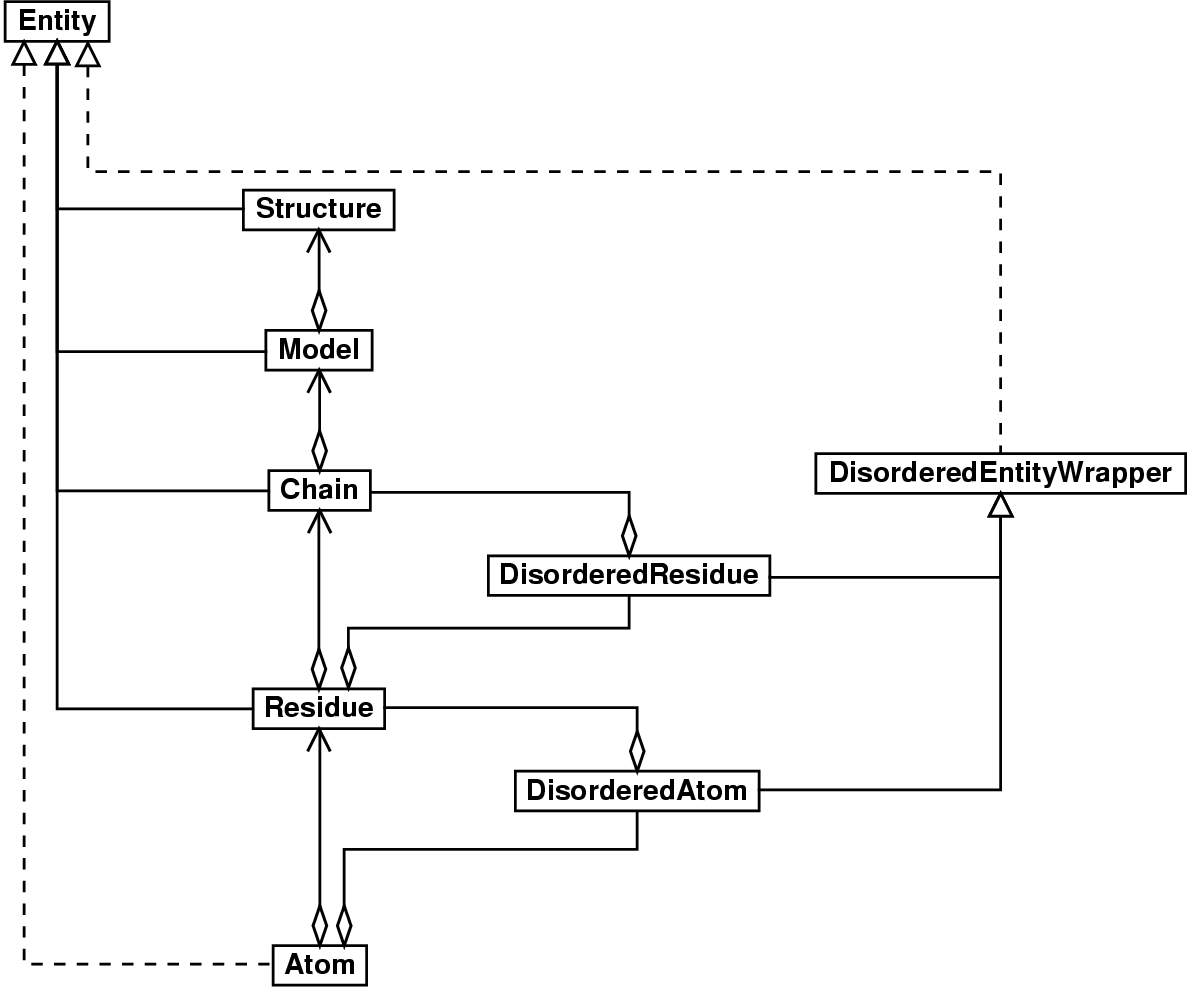
\includegraphics[width=6cm]{smcra}
\end{center}

\end{frame}

\begin{frame}[containsverbatim]
\frametitle{PDB parsing example}
\scriptsize
\begin{lstlisting}
>>> from Bio.PDB.PDBParser import PDBParser
>>> parser=PDBParser()
>>> structure=parser.get_structure("test","1WQ1.pdb")
>>> structure.get_list()
[<Model id=0>]
>>> model=structure[0]
>>> model.get_list()
[<Chain id=R>, <Chain id=G>]
>>> chain=model["R"]
>>> chain.get_list()
[<Residue MET het=  resseq=1 icode= >, <Residue THR het=  resseq=2 icode= >, <Residue GLU het=  resseq=3 icode= >, <Residue TYR het=  resseq=4 icode= >, <Residue LYS het=  resseq=5 icode= >
\end{lstlisting}
\normalsize
\end{frame}

\begin{frame}[containsverbatim]
\frametitle{Retrieving a PDB file}
\begin{lstlisting}
>>> from Bio.PDB import PDBList
>>> pdbl=PDBList()
>>> pdbl.retrieve_pdb_file('5P21')
retrieving ftp://ftp.wwpdb.org/pub/pdb/data/structures/divided/pdb/p2/pdb5p21.ent.gz
'/Users/jordivilla/merda/p2/pdb5p21.ent'
\end{lstlisting}
\url{http://www.biopython.org/DIST/docs/cookbook/biopdb_faq.pdf}
or:
\begin{lstlisting}
import urllib
def fetch_pdb(id):
  url = 'http://www.rcsb.org/pdb/files/%s.pdb' % id
  return urllib.urlopen(url).read()
\end{lstlisting}
\end{frame}

\section{Graphics}

\begin{frame}[containsverbatim]
\frametitle{Plotting with Python}
Matplotlib is the reference tool for plotting 2D data in Python. iPython has a "pylab" mode specific for interacting with matplotlib.

\url{http://wiki.python.org/moin/NumericAndScientific/Plotting}
\url{https://matplotlib.org/stable/tutorials/index.html}

\begin{lstlisting}
>>> from pylab import randn, hist
>>> x = randn(10000)
>>> hist(x, 100)
\end{lstlisting}
The pylab mode offers interaction similar to Matlab.
\url{http://matplotlib.sourceforge.net/}
Check also \url{http://gnuplot-py.sourceforge.net/}
\end{frame}

\begin{frame}[containsverbatim]
\frametitle{pyplot}
\url{https://www.tutorialspoint.com/matplotlib/matplotlib_pylab_module.htm}
\begin{lstlisting}
import matplotlib.pyplot as plt
plt.plot([1,2,3])
plt.ylabel('some numbers')
plt.show()
\end{lstlisting}
\begin{lstlisting}
import matplotlib.pyplot as plt
plt.plot([1,2,3,4], [1,4,9,16], 'ro')
plt.axis([0, 6, 0, 20])
\end{lstlisting}
\end{frame}

\begin{frame}[containsverbatim]
\frametitle{RPy}
\url{http://rpy.sourceforge.net/}
\begin{lstlisting}
>>> from rpy import *
>>>
>>> degrees = 4
>>> grid = r.seq(0, 10, length=100)
>>> values = [r.dchisq(x, degrees) for x in grid]
>>> r.par(ann=0)
>>> r.plot(grid, values, type='lines')
\end{lstlisting}
\end{frame}

\begin{frame}[containsverbatim]
\frametitle{working with numpy arrays}
\begin{lstlisting}
import numpy as np
import matplotlib.pyplot as plt

# evenly sampled time at 200ms intervals
t = np.arange(0., 5., 0.2)

# red dashes, blue squares and green triangles
plt.plot(t, t, 'r--', t, t**2, 'bs', t, t**3, 'g^')
\end{lstlisting}
\end{frame}


\section{CGI scripting}

\begin{frame}[containsverbatim]
\frametitle{Even before talking on CGI}
\begin{lstlisting}
import urllib

fwcURL = "http://cbbl.imim.es"

try:
   print ("Going to Web for data")
   fwcall = urllib.urlopen(fwcURL).read()
   print ("Successful")
   print ("Will now print all of the data to screen")
   print ("fwcall = ", fwcall)
except:
   print ("Could not obtain data from Web")
\end{lstlisting}
\end{frame}


\begin{frame}[containsverbatim]
\frametitle{Even before talking on CGI}
\small
\begin{lstlisting}
>>> import urllib2
>>> for line in urllib2.urlopen('http://tycho.usno.navy.mil/cgi-bin/timer.pl'):
...     if 'EST' in line or 'EDT' in line:  # look for Eastern Time
...         print (line)

<BR>Nov. 25, 09:43:32 PM EST

>>> import smtplib
>>> server = smtplib.SMTP('localhost')
>>> server.sendmail('soothsayer@example.org', 'jcaesar@example.org',
... """To: jcaesar@example.org
... From: soothsayer@example.org
...
... Beware the Ides of March.
... """)
>>> server.quit()
\end{lstlisting}
\normalsize
\end{frame}

\begin{frame}[containsverbatim]
\begin{lstlisting}
#!/usr/bin/env python

import cgi
print ("Content-Type: text/html\n")

print (""")
<HTML>
<HEAD>
<TITLE>Hello World</TITLE>
</HEAD>
<BODY>
<H1>Greetings</H1>
</BODY>
</HTML>
"""
\end{lstlisting}
\end{frame}

\section{Packaging}

\begin{frame}
\frametitle{Interface design}
\begin{enumerate}
\item Encapsulation
\item Generalization
\item Interface design
\item Refactoring
\end{enumerate}
\end{frame}

\section{Extensions}

\begin{frame}

\frametitle{Extending/embedding Python}
Python provides bindings to other languages that allow for powerful large project building. Check
\url{http://docs.python.org/extending/index.html}
for general information.
\end{frame}

\section{Glossary}

\begin{frame}[allowframebreaks]
\frametitle{Glossary}
\tiny
\begin{description}
\item[problem solving] The process of formulating a problem, finding a solution, and expressing the solution. 
\item[high-level language] A programming language like Python that is designed to be easy for humans to read and write. 
\item[low-level language] A programming language that is designed to be easy for a computer to execute; also called "machine language" or "assembly language" 
\item[portability] A property of a program that can run on more than one kind of computer. 
\item[interpret] To execute a program in a high-level language by translating it one line at a time. 
\item[compile] To translate a program written in a high-level language into a low-level language all at once, in preparation for later execution. 
\item[source code] A program in a high-level language before being compiled. 
\item[ob ject code] The output of the compiler after it translates the program. 
\item[executable] Another name for ob ject code that is ready to be executed. 
\item[prompt] Characters displayed by the interpreter to indicate that it is ready to take input from the user. 
\item[script] A program stored in a file (usually one that will be interpreted).
\item[program] A set of instructions that specifies a computation. 
\item[algorithm] A general process for solving a category of problems. 
\item[bug] An error in a program. 
\item[debugging] The process of finding and removing any of the three kinds of programming errors. 
\item[syntax] The structure of a program. 
\item[syntax error] An error in a program that makes it impossible to parse (and therefore impossible to interpret). 
\item[exception] An error that is detected while the program is running. 
\item[semantics] The meaning of a program. 
\item[semantic error] An error in a program that makes it do something other than what the programmer intended. 
\item[natural language] Any one of the languages that people speak that evolved naturally. 
\item[formal language] Any one of the languages that people have designed for specific purposes, such as representing mathematical ideas or computer programs; all programming languages are formal languages. 
\item[token] One of the basic elements of the syntactic structure of a program, analogous to a word in a natural language. 
\item[parse] To examine a program and analyze the syntactic structure. 
\item[print statement] An instruction that causes the Python interpreter to display a value on the screen.
\item[instance] A member of a set. 
\item[loop] A part of a program that can execute repeatedly. 
\item[encapsulation] The process of transforming a sequence of statements into a function definition. 
\item[generalization] The process of replacing something unnecessarily specific (like a number) with something appropriately general (like a variable or parameter). 
\item[interface] A description of how to use a function, including the name and descriptions of the arguments and return value. 
\item[development plan] A process for writing programs. 
\item[docstring] A string that appears in a function definition to document the function's interface. 
\end{description}
\normalsize
\end{frame}

\section{Annexes}

\begin{frame}
\frametitle{This document's history}
\begin{enumerate}
\item 2007 : Original version by Michael A. Johnston
\item 2008 : modifications and examples added by JVF
\item 2010-: \LaTeX2e\ version and extensions by JVF
\end{enumerate}
\end{frame}

\begin{frame}
\frametitle{Sources}
\small
\begin{itemize}
\item Style guide for Python code \url{http://www.python.org/dev/peps/pep-0008/}
\item Library: \url{http://docs.python.org/library/}
\item \url{http://www.thinkpython.com}
\item \url{http://diveintopython.org/toc/index.html}
\item \url{http://docs.python.org/tutorial/introduction.html}
\item \url{http://openbookproject.net/thinkcs/python/english2e/}
\item \url{http://www.awaretek.com/tutorials.html}
\item \url{http://code.google.com/edu/languages/google-python-class/}
\item \url{http://www.sthurlow.com/python/}
\end{itemize}
\normalsize
\end{frame}

\end{document}
